\documentclass[a4paper,12pt]{article}
\usepackage{amssymb}
\usepackage{amsmath}
\usepackage[utf8]{inputenc} % Umlaute
\usepackage[ngerman]{babel} % Umlaute
\usepackage[T1]{fontenc}    % Umlaute
\usepackage[margin=2.5cm]{geometry}
\usepackage{booktabs}
\usepackage{lmodern}

% Notwendig für Links im Text
\usepackage{hyperref}

% glossar, see http://en.wikibooks.org/wiki/LaTeX/Glossary
% muss NACH hyperref geladen werden, sonst funktionieren die Links nicht
\usepackage{glossaries}

% Kompatibilität
\ifx\pdftexversion\undefined
\usepackage[dvips]{graphicx}
\else
\usepackage[pdftex]{graphicx}
\DeclareGraphicsRule{*}{mps}{*}{}
\fi

\makeglossaries

%%%%%%%%%%%%%%%%%%%%%%%%%%%%%%%%%%%%%%%%%%%%%%%%%%%%%%%%%%%%%%%%%%%%%%
% Variablen                                 						 %
%%%%%%%%%%%%%%%%%%%%%%%%%%%%%%%%%%%%%%%%%%%%%%%%%%%%%%%%%%%%%%%%%%%%%%
\newcommand{\authorName}{Tec O'Brain (Entwickler: David Höglinger, Jan Ettrich, Erwin Müller, Benedikt Rittner, Valentin Quapil)}
\newcommand{\auftraggeber}{Karlsruhe Institute of Technology (Teco)}
\newcommand{\auftragnehmer}{\authorName}
\newcommand{\projektName}{Pflichtenheft Earables}
\newcommand{\tags}{\authorName, Pflichtenheft, KIT, Informatik, PSE}
\newcommand{\glossarName}{Glossar}
\title{\projektName}
\date{\today}

%%%%%%%%%%%%%%%%%%%%%%%%%%%%%%%%%%%%%%%%%%%%%%%%%%%%%%%%%%%%%%%%%%%%%%
% PDF Meta information                                 				 %
%%%%%%%%%%%%%%%%%%%%%%%%%%%%%%%%%%%%%%%%%%%%%%%%%%%%%%%%%%%%%%%%%%%%%%
\hypersetup{
  pdfauthor   = {\authorName},
  pdfkeywords = {\tags},
  pdftitle    = {\projektName)}
}

%%%%%%%%%%%%%%%%%%%%%%%%%%%%%%%%%%%%%%%%%%%%%%%%%%%%%%%%%%%%%%%%%%%%%%
% Create a shorter version for tables. DO NOT CHANGE               	 %
%%%%%%%%%%%%%%%%%%%%%%%%%%%%%%%%%%%%%%%%%%%%%%%%%%%%%%%%%%%%%%%%%%%%%%
\newcommand\addrow[2]{#1 &#2\\ }

\newcommand\addheading[2]{#1 &#2\\ \hline}
\newcommand\tabularhead{\begin{tabular}{lp{13cm}}
\hline
}

\newcommand\addmulrow[2]{ \begin{minipage}[t][][t]{2.5cm}#1\end{minipage}%
   &\begin{minipage}[t][][t]{8cm}
    \begin{enumerate} #2   \end{enumerate}
    \end{minipage}\\ }

\newenvironment{usecase}{\tabularhead}
{\hline\end{tabular}}

\usepackage{microtype}
%%%%%%%%%%%%%%%%%%%%%%%%%%%%%%%%%%%%%%%%%%%%%%%%%%%%%%%%%%%%%%%%%%%%%%
% GLOSSARY ENTRIES                 	                              	 %
%%%%%%%%%%%%%%%%%%%%%%%%%%%%%%%%%%%%%%%%%%%%%%%%%%%%%%%%%%%%%%%%%%%%%%

\newglossaryentry{Echtzeit}{name=Echtzeit, description={Bereitstellen/Anzeigen von Daten mit einer durch die Verarbeitung bedingten Verzögerung von bis zu ca. 2 Sekunden zwischen dem Anfallen der (Roh-)Daten und der Ausgabe bzw. Visualisierung.}}
\newglossaryentry{Vorgang}{name=Vorgang, description={Als Vorgang wird in diesem Pflichtenheft bezeichnet, wenn ein Modus ausgewählt ist und Start gedrückt wurde. Der Vorgang endet mit dem Drücken von Stopp bzw. wird mit dem Wechseln des Modus.}}
\newglossaryentry{BLE}{name=BLE, description={Bluetooth Low Energy ist eine Technologie, die Teil des Industriestandards Bluetooth ist und eine energiesparende, kabellose Kommunikation zwischen Geräten in einer Entfernung von bis zu ca. 10 Metern ermöglicht.}}
\newglossaryentry{Wearable Computer}{name=Wearable Computer, description={Unter dem Begriff Wearable Computer versteht man Computersysteme, die am Körper, unter der Kleidung oder als Implantat unter der Haut getragen werden können.}}
\newglossaryentry{IMU}{name=6-Achsen IMU, description={Ein 6-Achsen IMU ist ein Beschleunigungssensor mit Gyroskop.}}
\newglossaryentry{GUI}{name=GUI, description={GUI ist die Abkürzung für den englischen Begriff \glqq graphical user interface\grqq . Sie ist die Schnittstelle zwischen Mensch und Maschine und ermöglicht dem Nutzer die Eingabe/Steuerung, der Maschine.}}
\newglossaryentry{Cross-Platform Bibliothek}{name=Cross-Platform Bibliothek, description={Eine Cross-Platform Bibliothek ist nichts weiter als eine Bibliothek die auf Rechnersystemen mit verschiedener Architektur laufen kann.}}
\newglossaryentry{Steuerungsparameter}{name=Steuerungsparameter, description={Unter Steuerungsparametern fassen wir die Länge der Verbindungsintervalle zwischen Earables und Smartphone sowie die Abtastrate und den Wertebereich von integriertem Gyroskop und Beschleunigungssensor zusammen.}}
\newglossaryentry{Schrittfrequenz}{name=Schrittfrequenz, description={Die Schrittfrequenz gibt an wie viele Schritte pro Zeiteinheit gemacht werden.}}
\newglossaryentry{Rohdaten}{name=Rohdaten, description={Als Rohdaten werden unverarbeitete Daten bezeichnet.}}
\newglossaryentry{TTS}{name=Text-To-Speech, description={Ein Text-to-Speech-System (TTS) (oder Vorleseautomat) wandelt Fließtext in eine akustische Sprachausgabe um. Dabei erfolgt diese auf Deutsch oder auf Englisch, abhängig davon, was als Sprache eingestellt ist.}}
\newglossaryentry{Earables}{name=Earables, description={Eine Zusammenschließung des Wortes Wearable und Earphone. Dabei handelt es sich um Kopfhörer, die mit Sensoren ausgestattet sind.}}
\newglossaryentry{Vorgangsdaten}{name=Vorgangsdaten, description={Daten, die bei der Ausführung eines Vorgangs gespeichert werden (z.B. Schritte, Sit-ups,\dots).}}


%%%%%%%%%%%%%%%%%%%%%%%%%%%%%%%%%%%%%%%%%%%%%%%%%%%%%%%%%%%%%%%%%%%%%%
% THE DOCUMENT BEGINS             	                              	 %
%%%%%%%%%%%%%%%%%%%%%%%%%%%%%%%%%%%%%%%%%%%%%%%%%%%%%%%%%%%%%%%%%%%%%%
\begin{document}
 \pagenumbering{roman}
 \begin{titlepage}
\maketitle
\thispagestyle{empty} % no page number

\begin{verbatim}












\end{verbatim}


  \begin{tabular}[t]{p{4 cm}p{8 cm}}
	Projekt:       & \projektName \\[1.2ex]
	Auftraggeber:  & \auftraggeber\\[1.2ex]
	Auftragnehmer: & \auftragnehmer\\[1.2ex]
  \end{tabular}


\begin{tabular}[t]{|p{4 cm}|p{8 cm}|}
\hline
\textbf{Datum} & \textbf{Autor(en)} \\
\hline
\hline
\today & \authorName \\
\hline
\end{tabular}
\end{titlepage}
         % Deckblatt.tex laden und einfügen
 \setcounter{page}{2}
 \tableofcontents          % Inhaltsverzeichnis ausgeben
 \clearpage
 \pagenumbering{arabic}


\section{Einleitung}
\Gls{Earables} gehören zu den \Gls{Wearable Computer}, sie sind also nichts anderes als intelligente Kopfhörer. Je nachdem wie sie ausgestattet werden bringen sie die unterschiedlichsten Funktionen mit sich. Neben der klassischen Ausstattung von Lautsprechern, Mikrophon und \gls{BLE} besitzen sie in unserem Fall zusätzlich eine \Gls{IMU}. Mit ihrer Hilfe ist man in der Lage die Bewegungen des Nutzers zu erkennen und aufzuzeichnen, um mit den gewonnenen Messdaten  beispielsweise die \Gls{Schrittfrequenz} zu messen.  \Gls{Earables} bilden also eine Schnittstelle zwischen Mensch und Computer. Da sie kaum von normalen Bluetooth Kopfhörern zu unterscheiden sind, haben sie bereits jetzt eine hohe soziale Akzeptanz in der Gesellschaft erlangt, im Gegensatz zu beispielsweise Smartglasses. Mit der Entwicklung und Forschung dieser Art von \Gls{Earables} beschäftigt sich das globale eSense Projekt von Nokia Bell Labs in Zusammenarbeit mit dem TECO. Hier wird gemeinsam nach möglichen Anwendungsfällen der \Gls{Earables} gesucht, wodurch auch dieses Projekt initiiert wurde.
\section{Zielbestimmung}
Die Ziele dieses Projektes lassen sich in drei Bereiche gliedern:
\begin{enumerate}

  \item Es soll eine \Gls{Cross-Platform Bibliothek} (Android/IOS) für die \Gls{Earables} der Plattform eSense entwickelt werden mit der es möglich ist, die gemessenen Rohdaten der \Gls{Earables} aufzuzeichnen und verschiedene \Gls{Steuerungsparameter} zu verändern.
  
  \item Es soll ein Erweiterungsmodul entwickelt werden, mit dem die übermittelten  \Gls{Rohdaten} automatisch verarbeitet und ausgewertet werden, um so festzustellen, ob der Nutzer gerade läuft oder steht.
  
  \item Es soll eine App mit einer \Gls{GUI} entwickelt werden, die über verschiedene Modi verfügt. Einer dieser Modi soll anzeigen ob der Nutzer gerade läuft oder steht. Die \gls{Schrittfrequenz} des Nutzers und die Anzahl der zurückgelegten Schritte sollen auch angezeigt werden.

\end{enumerate}

\subsection{Musskriterien}

  \begin{itemize}
    \item Die \Gls{Cross-Platform Bibliothek} soll in der Lage sein, die gesammelten Daten der \Gls{Earables} aufzuzeichnen.
    \item Die \Gls{Cross-Platform Bibliothek} soll in der Lage sein die verschiedenen \Gls{Steuerungsparameter} zu verändern.
    \item Das Erweiterungsmodul soll erkennen ob der Nutzer gerade \glqq läuft\grqq{}oder \glqq steht\grqq.
    \item Das Erweiterungsmodul soll die \gls{Schrittfrequenz} und die Schrittanzahl ermitteln können.
    \item Die App soll anzeigen können ob der Nutzer gerade läuft oder steht.
    \item Die App soll die aktuelle Schrittfrequenz anzeigen.
    \item In der App wird die Anzahl der gelaufenen Schritte gespeichert.
    \item Die \Gls{GUI} der App muss so benutzerfreundlich gestaltet werden, dass der Benutzer intuitiv weiß wie man die \Gls{Steuerungsparameter} der \Gls{Earables} verändert.
  \end{itemize}
\subsection{Wunschkriterien}
  \begin{itemize}
    \item Die App soll über drei weitere Modi verfügen.
      \begin{itemize}
        \item Im Modus \glqq Zählmodus\grqq{} zählt die App wie viele Liegestütze oder Sit-ups der Nutzer macht.
        \item Im Modus \glqq Lauschen\&Agieren\grqq{} kann der Nutzer seinen eigenen Trainingsablaufplan erstellen, welcher dann über \Gls{TTS} ausgegeben wird.
        \item Im Modus \glqq Musikmodus\grqq{} wird Musik abgespielt, wenn der Nutzer läuft und automatisch pausiert, wenn der Nutzer steht. Sobald der Nutzer weiter läuft wird die Musik auch wieder weiterlaufen.
      \end{itemize}
    \item Die App soll die zurückgelegte Distanz anzeigen.
    \item Während der \glqq Laufmodus\grqq{} aktiv ist, werden die aktuelle Schrittanzahl und die zurückgelegte Distanz live angezeigt.
    \item Wenn kein Laufvorgang aktiv ist, werden im Laufmodus die Daten (Schritte, Distanz) des letzten Datums angezeigt.
    \item Die App wird standardmäßig auf die Sprache des Smartphone eingestellt sein. Die Sprache kann in den Einstellungen auf Deutsch oder Englisch gewechselt werden. Sollte die Sprache des Smartphones nicht unterstützt werden wird standardmäßig Englisch verwendet. 
    \item Vorgangsdaten werden automatisch gespeichert; Importieren und Exportieren soll möglich sein.
  \end{itemize}
  \subsection{Abgrenzungskriterien}
  \begin{itemize}
    \item Es werden keine \Gls{Rohdaten} auf dem Smartphone des Nutzers gespeichert.
    \item Die Musik passt sich nicht der \Gls{Schrittfrequenz} des Nutzers an.
    \item Im Modus \glqq Zählen\grqq{} wird davon ausgegangen, dass der Nutzer wirklich nur Liegestützen oder Sit-ups macht. Das bewusste Austricksen des Systems durch andere Bewegungen wird nicht behandelt.
    \item Auf den \Gls{Earables} werden keine Vorgangsdaten gespeichert.
    \item Die Daten des Mikrophons werden weder aufgezeichnet noch ausgewertet.
  \end{itemize}
\clearpage
\section{Produkteinsatz}
Unser Produkt besteht aus drei Teilen (der Bibliothek, dazu das Erweiterungsmodul und der App), dementsprechend gibt es auch verschiedene Zielgruppen und Anwendungsbereiche.
  \subsection{Zielgruppe}
  \begin{itemize}
    \item\textsf{Bibliothek:} Softwareentwickler
    \item\textsf{Erweiterungsmodul:} Softwareentwickler
    \item\textsf{App:} Hobbysportler
  \end{itemize}
  \subsection{Anwendungsbereiche}
    \begin{itemize}
      \item\textsf{Bibliothek} 
      \begin{itemize}
        \item Softwareentwicklung für eSense Wearables 
      \end{itemize}
      \item\textsf{Erweiterungsmodul}
      \begin{itemize}
        \item Softwareentwicklung im Bereich Schritterkennung.
        \item Auswerten der von \Gls{Earables} aufgezeichneten Rohdaten für die Verwendung in einer App, z.B. im Bereich Fitness, aber auch als Nutzereingabe für andere interaktive Apps.
      \end{itemize}
      \item\textsf{App} Heimtraining, Sport, \dots
    \end{itemize}
  \subsection{Betriebsbedingungen der App} %% hier wollte David noch was hinzufügen
    \subsubsection{Physikalische Umgebung}
      Die physikalische Umgebung der Anwendung ist hardwareabhängig.
    \subsubsection{Sonstiges}
    \begin{itemize}
      \item \textsf{Betriebsdauer:} \glqq Akkuabhängig\grqq, keine weitere Grenzen.
      \item \textsf{Qualifikation des Nutzers:} Sollte Sportübungen selbstständig ausführen können.
      \item \textsf{Vordergrund:} Die App muss im Vordergrund laufen, damit die Vorgänge funktionieren, siehe /NF065/.
    \end{itemize}
\clearpage
\section{Produktumgebung}
Es handelt sich bei der App um eine Smartphoneanwendung, daher wird das Produkt als Installationspaket ausgeliefert. Außerdem setzen wir bestimmte Hardware- und Softwarebedingungen voraus.
\subsection{Hardware} 
\begin{itemize}
  \item \textsf{Minimale Anforderungen:} Smartphone mit \Gls{BLE} Unterstützung. 
  \item \textsf{Leistungsanforderung:} Das Smartphone sollte mindestens 1 GB Arbeitsspeicher besitzen.
  \item \textsf{Speicheranforderung:} Das Smartphone sollte mindestens 100 MB Speicherplatz zur Verfügung haben.
\end{itemize}

\subsection{Software} 
	\textsf{Betriebssystem:} Unterstützung von Android ab Version 7 und iOS ab Version 10.

\vspace{1cm}
\section{Funktionale Anforderungen}
Die Funktionalen Anforderungen gliedern sich in einen Pflichtteil (was unbedingt umgesetzt werden muss) und einen Wunschteil (Anforderungen, die umgesetzt werden sollten, aber nicht essenziell sind). Die Funktionalen Anforderungen spezifizieren auf Ebene der Bibliothek, des Erweiterungsmoduls und der App, welche Funktionen umgesetzt werden müssen bzw. können. 
  \subsection{Mussanforderungen}
    \subsubsection{Bibliothek}
    \begin{itemize}
      \item[/F010/] Gemessene \Gls{Rohdaten} des \Gls{IMU} in \Gls{Echtzeit} zur Verfügung stellen.
      \item[/F030/] \Gls{Steuerungsparameter} (Abtastrate, Wertebereich Gyroskop/Beschleunigungssensor, Tiefpassfilter) ändern. %%die einzigen "Messparameter" die wir ändern können sind die abtastrate und die start/stop des samplings
      \item[/F040/] Die Datenaufnahme des \Gls{IMU} starten und stoppen.
    \end{itemize}
    \subsubsection{Erweiterungsmodul}
     Auswertung der ausgelesenen Daten:
     \begin{itemize}
      \item[/F060/] \textsf{Schritterkennung:} Es wird erkannt ob der Nutzer einen Schritt tätigt.
      \item[/F061/] \textsf{Schrittfrequenzerkennung:} Während der Nutzer läuft wird die Schrittfrequenz ermittelt.
      \item[/F062/] \textsf{Schrittanzahl wird gezählt:} Die Schritte des Nutzers werden gezählt.
      \item[/F063/] \textsf{Berechnung Distanz:} Die zurückgelegte Distanz des Nutzers soll berechnet werden können.
    \end{itemize}
    \subsubsection{App}
      \begin{itemize}
      \item[/F070/] \textsf{App starten:} Der Nutzer kann die App über sein Smartphone starten. Die App startet im Laufmodus.
      \item[/F075/] \textsf{Vorgang starten:} Der Nutzer kann den modusspezifischen \Gls{Vorgang} starten. Dann wird der Modus seiner Beschreibung nach aktiv ausgeführt.
      \item[/F080/] \textsf{Vorgang stoppen:} Der Nutzer kann den modusspezifischen \Gls{Vorgang} stoppen.
      \item[/F085/] \textsf{Resultat anzeigen:} Nach Stoppen wird das Vorgangsresultat angezeigt.
      \item[/F090/] \textsf{Modus wechseln:} Der Nutzer kann zwischen Modi über ein einblendbares Menü wechseln.
      \item[/F100/] \textsf{Laufmodus:} Liveanzeige, ob der Nutzer gerade \glqq läuft\grqq{} oder \glqq steht\grqq{}, mit Hilfe von /F060/.
      \item[/F101/] \textsf {Schrittfrequenz anzeigen:} Im Modus \glqq{}Laufmodus\grqq{} wird die Schrittfrequenz des Nutzers angezeigt, sobald der Vorgang gestartet wird. Die Schrittfrequenz wird mit Hilfe von /F061/ ermittelt.
      \item[/F102/] \textsf {Schrittanzahl anzeigen:} Im Modus \glqq{}Laufmodus\grqq{} wird die Schrittanzahl des Nutzers angezeigt, sobald der Vorgang gestartet wird. Die Schrittanzahl wird mit Hilfe von /F062/ ermittelt. Die Schrittzählung beginnt/endet mit dem Starten/Stoppen des Vorgangs.
      \item[/F103/] \textsf{Schrittanzahl Speichern:} Die App speichert die Schrittanzahl pro Tag für die letzten 30 Tage an denen der Laufmodus aktiv war.
      \item[/F104/] \textsf{Ergebnisse des letzten Vorgangs anzeigen:} Wenn sich die App im Laufmodus befindet und der Vorgang noch nicht gestartet wurde, wird angezeigt wie weit der Nutzer beim letzten Vorgang gelaufen ist und wie viele Schritte er gemacht hat. Falls es noch keine Einträge gibt werden Nullwerte angezeigt.
      \item[/F140/] \textsf{BLE-Verbindung herstellen:} Sobald der Nutzer die App startet erscheint ein Pop-up Fenster, über das der Nutzer sein Smartphone mit den \gls{Earables} verbinden kann. Ohne BLE-Verbindung kann der Nutzer keinen Vorgang starten.
      \item[/F150/] \textsf{BLE-Verbindung unterbrochen:} Falls die App die Verbindung zu den \gls{Earables} verlieren sollte, erscheint wieder das Pop-up Fenster aus /F140/.
      \item[/F160/] \textsf{BLE-Verbindung nicht notwendig:} Der Nutzer kann das Pop-up Fenster aus /F140/ wegklicken.
      \item[/F165/] \textsf{BLE-Verbindung später herstellen:} Falls der Nutzer keine BLE-Verbindung mit den \gls{Earables} besitzt und einen Vorgang startet, so erscheint zunächst das Pop-up Fenster aus /F140/.
    \end{itemize}
  \subsection{Wunschanforderungen}
    \subsubsection{Erweiterungsmodul}
      \textsf{Weitere Datenauswertung:}
      \begin{itemize}
      \item[/F170/] \textsf{Erkennung Sit-ups} Das Erweiterungsmodul kann erkennen, ob der Nutzer Sit-ups macht.
      \item[/F180/] \textsf{Erkennung Liegestütze} Das Erweiterungsmodul kann erkennen, ob der Nutzer Liegestütze macht.
      \end{itemize} 
    \subsubsection{App}
    \textsf{Weitere Modi:}
    \begin{itemize}

       
       
        \item[/F200/] \textsf{Zählmodus:} Zählen von Liegestützen oder Sit-ups mit Hilfe von /F170/ und /F180/.
        \item[/F210/] \textsf{Start/Stopp Musikmodus:} Musik stoppt wenn Nutzer stehen bleibt, läuft wenn der Nutzer läuft. Bei diesem Modus werden keine Resultate angezeigt.
      
 	    \item[/F220/] \textsf{Modus \glqq Lauschen\&Agieren\grqq:}
 	    \begin{itemize}
        \item[/F221/]Der Nutzer kann sich einen Trainingsablaufplan zusammenstellen, indem er in einer Liste Aktivitäten hinzufügt (Liegestütze, Sit-ups, Laufen, Pausenzeit). 
        \item[/F222/] Der Nutzer erhält Sprachanweisungen per \Gls{TTS} für die nächste Übung während des Vorgangs. Die nächste Sprachanweisung kommt erst, wenn der Nutzer die aktuelle Aktivität vollständig beendet hat.
        \item[/F223/] Neben dem Vorgangsresultat wird dem Nutzer nach Beenden des Vorgangs auch die Zeit angezeigt, in der er die Aktivitäten absolviert hat.
        \item[/F224/] Die Sprachanweisung erfolgt in der Sprache der in-App Einstellungen.
    	\end{itemize}
   \end{itemize}
		\textsf{Einstellungen:}
   \begin{itemize}
        \item[/F250/] Der Nutzer kann seinen Namen in den Einstellungen ändern.
        \item[/F260/] Der Nutzer kann die Sprache der App verändern. (Möglichkeiten sind Deutsch und Englisch)
        \item[/F265/] Die Sprache der App wird sich bei der Erstnutzung an die Systemsprache des Nutzers anpassen. Standardmäßig ist dies Englisch, bei deutscher Systemsprache wird Deutsch eingestellt.
        \item[/F270/] Der Nutzer kann die gespeicherten \Gls{Vorgangsdaten} löschen.
        \item[/F280/] Der Nutzer kann die \Gls{Steuerungsparameter} anpassen. 
        \item[/F285/] Der Nutzer kann die Schrittlänge für die Distanzmessung anpassen.
  	\end{itemize}
		\textsf{Sonstiges:}
	\begin{itemize}
        \item[/F290/] Aufforderung der Angabe von Name und Schrittlänge bei Erstnutzung.
        \item[/F300/] Der Nutzer kann in der App seine gesamten \Gls{Vorgangsdaten} exportieren, importieren und löschen. Dabei wird das CSV-Format genutzt. 
        \item[/F310/] Speicherung von Sit-ups, Liegestütze und Schrittanzahl für jeden Tag, an dem ein \Gls{Vorgang} aktiv war.
        \item[/F320/] Der Nutzer kann die gespeicherten Vorgangsdaten /F310/ der letzten 30 Tage, an denen mindestens ein Vorgang gestartet wurde, einsehen. 
  
  
      \end{itemize}
\vspace{1cm}
\section{Produktdaten}
Die App soll dem Nutzer die Möglichkeit zur Verfügung stellen, seine Trainingsdaten auch nach Beenden der App weiterhin zu Nutzen. Zu diesem Zweck werden die Trainingsdaten auf dem Smartphone gespeichert; immer sobald ein Vorgang abgeschlossen ist.
\begin{itemize}
	\item[/PD010/] Es werden keine rohen Messdaten gespeichert.
	\item[/PD020/] Die Einstellungen (Sprache, \Gls{Steuerungsparameter}, Benutzernamen) sind zu speichern. 
	\item[/PD030/] Die gesammelten \Gls{Vorgangsdaten} werden auf dem Gerät in einer Datenbank gespeichert, siehe /F310/.
\end{itemize}

\vspace{1cm}
\section{Nichtfunktionale Anforderungen}
Wie unter dem Punkt Qualitätszielbestimmungen aufgeführt, legen wir unsere Priorität vor allem auf Korrektheit und Benutzerfreundlichkeit. Um die Benutzerfreundlichkeit zu gewährleisten, werden hier einige Anforderungen an die Stabilität, den Speicherplatz und das Laufzeitverhalten gestellt. Für das korrekte Funktionieren werden weitere allgemeine Anforderungen formuliert.
\subsection{Allgemein}
\begin{itemize}
  \item[/NF010/] Beim Änderung der \Gls{Steuerungsparameter} (/F030/) soll die Datenaufnahme der \Gls{IMU} gestoppt werden.
  \item[/NF020/] Beim Wechseln zwischen Modi (/F090/) soll der aktuelle Vorgang terminiert werden.
  \item[/NF030/] Nach dem Ändern der Sprache der App (/F260/) muss die App neu gestartet werden.
  \item[/NF040/] Bei nicht sinnvollen Angaben (z.B. negativen Werten in /F221/) wird das Starten des Vorgangs verhindert.
  \item[/NF050/] Bei Namensänderung (/F250/) werden gespeicherte Daten (siehe /F300/) nicht verändert.
  \item[/NF060/] Bei Namensgebung sind nur Groß- und Kleinbuchstaben ohne Umlaute und Sonderzeichen erlaubt.
  \item[/NF065/] Gerät die App durch Minimieren oder Ausschalten des Smartphone Bildschirms in den Hintergrund, wird der aktuelle Vorgang terminiert.
  \item[/NF066/] Earables und Smartphone sollten nicht über zehn Meter voneinander entfernt werden, sodass eine Bluetooth-Verbindung möglich ist. 
  \item[/NF067/] Beim Starten der App /F070/ wird der Vorgang im Laufmodus nicht automatisch gestartet.
\end{itemize}
\subsection{Stabilität}
\begin{itemize}
  \item[/NF070/] Die App soll bei herkömmlicher Nutzung nicht öfter als zweimal bei zehnmaliger Benutzung abstürzen. 
\end{itemize}
\subsection{Speicherplatz}
\begin{itemize}
  \item[/NF080/] Die App soll eine Größe von 100 MB nicht überschreiten. 
  \item[/NF090/] Die gespeicherten Daten sollen nicht mehr als 50 MB umfassen. 
\end{itemize}
\subsection{Laufzeitverhalten}
\begin{itemize}
  \item[/NF100/] Die Liveanzeige des Laufmodus (/F100/) soll maximal eine Verzögerung von zwei Sekunden aufweisen. 
  \item[/NF110/] Der Start eines Vorgangs nach seiner Auswahl (/F080/) soll nicht länger als zwei Sekunden benötigen. 
  \item[/NF120/] Die Einblendung des Vorgangsresultats (/F130/) soll nicht länger als zwei Sekunden benötigen.
  \item[/NF130/] Der Verbindungsaufbau mit den \Gls{Earables} darf nicht länger als 5 Sekunden dauern.

\end{itemize}
\section{Systemmodelle der App}
%%TODO Jan!!
  \subsection{Architekturdiagramm}
  \begin{center}
  	\vspace{100px}
  	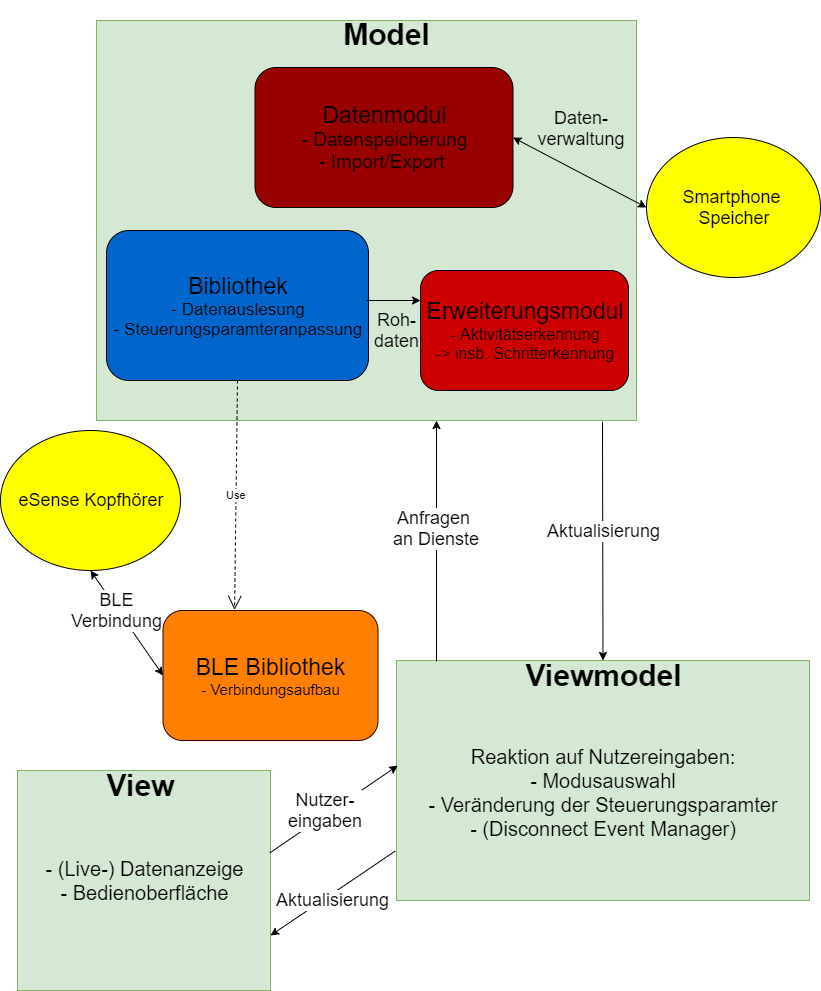
\includegraphics[width=0.8\textwidth]{./Diagramme/Achi5.png}
  \end{center}
  \clearpage %%sieht sonst noch zerrissener aus;    Gehts nicht irgendwie schöner? Sodass das Diagramm ganz oben quasi anliegt?
  \subsection{Kurze Erläuterung zum Architekturdiagramm}
  Wir haben uns bei der Architekturdiagramm für \textsf{Model-View-Viewmodel}, eine Spezialisierung  des Entwurfsmusters Model-View-Controller, entschieden.
  Dabei gibt es folgende Komponenten:
  \begin{itemize}
    \item \textsf{\glqq View\grqq{}} enthält alle grafisch angezeigten Elemente, also die Datenanzeige und Bedienoberfläche der App.
    \item {\textsf{\glqq Model\grqq{}} enthält die Geschäftslogik der App und ist stark nach außen abgekapselt. In diesen Bereich fallen die meisten komplexen Teile der App, die als Dienste (Services) vom Viewmodel aus verwaltet werden sollen. Wesentlich sind dabei (vollständige Angabe im Entwurf): \begin{itemize}
      \item Die Verwaltung der anfallenden Produktdaten (Abruf und Bereitstellung der gespeicherten Daten in der Datenbank, im CSV-Format) über ein Datenmodul
      \item Die Bibliothek, die für die Kommunikation mit den \Gls{Earables} (Verbindungsaufbau, Start und Stopp des Samplings, Konfiguration der \Gls{Steuerungsparameter}, Auslesen der Sensordaten) zuständig ist. Dazu wird eine externe Bibliothek\footnote{https://github.com/xabre/xamarin-bluetooth-le} verwendet.
      \item Das Erweiterungsmodul, das sich um die Aktivitätserkennung kümmert. Dieses nutzt dabei die Schnittstellen der Bibliothek.
    \end{itemize}
    Die Services sind dabei jeweils unabhängig vom restlichen Model funktionsfähig und dadurch leichter testbar.}
    \item \textsf{\glqq Viewmodel\grqq{}} ist das Bindeglied zwischen View und Model. Es enthält die Logik der UI, wird also bei Benutzerinteraktion vom View aufgerufen. Es gibt dann die entsprechenden Anweisungen an das Model weiter. Darüber hinaus kümmert es sich darum, dass in bestimmten Fällen die Anzeige der App angepasst wird, zum Beispiel bei Verbindungsabbruch zu den \Gls{Earables}. 
    
  \end{itemize}
  Der Vorteil dieser Architektur ist eine klare Trennung von Benutzerinteraktion und Programmlogik sowie eine lose Kopplung zwischen einzelnen Funktionalitäten, was die Flexibilität und das modulare Testen deutlich erleichtert.
  \subsection{Use-Case-Diagramm}
  \begin{center}
	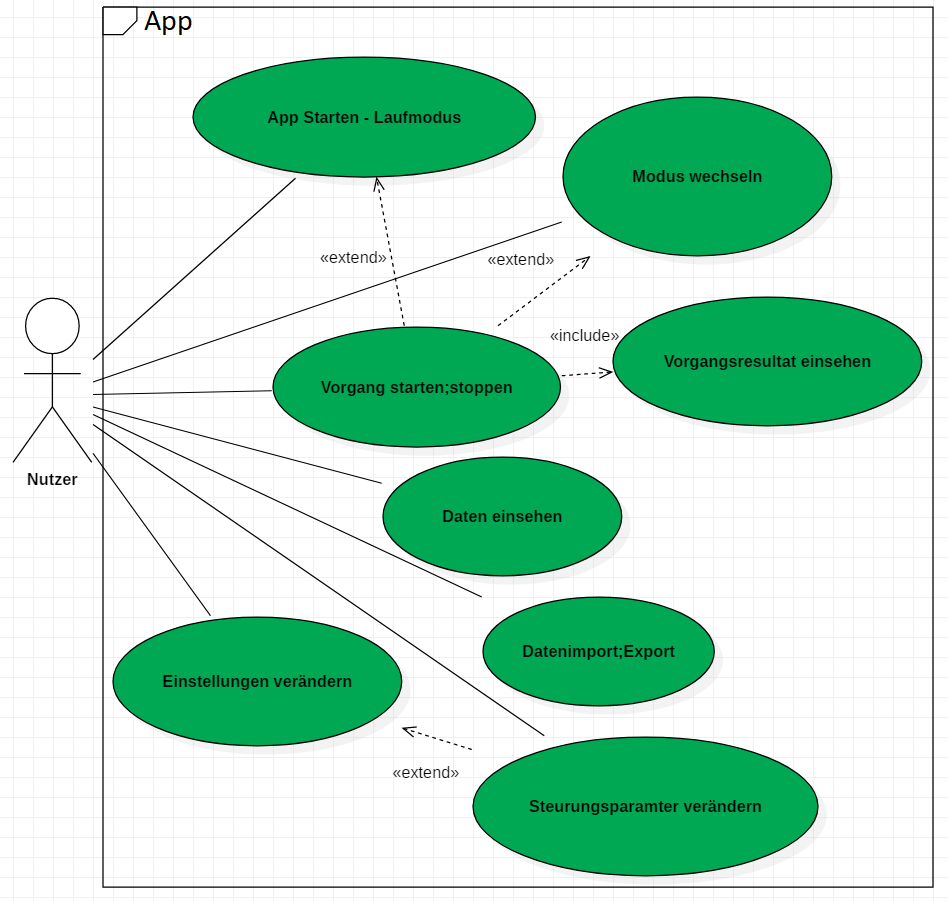
\includegraphics[width=0.8\textwidth]{./Diagramme/Use-CaseDiagramm.png} 
  \end{center}

\subsubsection{Beschreibung} 
Beim Starten der App landet der Nutzer automatisch im Laufmodus. Bevor ein Modus genutzt werden kann muss der Nutzer eine BLE Verbindung über ein Pop-up Fenster mit den \Gls{Earables} herstellen. Der Nutzer kann nun entweder den Modus wechseln oder einen \Gls{Vorgang} starten. Nach Beendigung oder Stoppen eines Vorgangs wird das Vorgangsresultat angezeigt. Der Nutzer kann außerdem vergangene Vorgangsdaten einsehen und diese auch importieren/exportieren. Das Ändern von Einstellungen der App und der \Gls{Steuerungsparameter} der \Gls{Earables} über die App ist ebenfalls möglich.
\section{Benutzeroberfläche}
\subsection{Einführung}
Die \Gls{GUI} wird durch die App realisiert. Dabei kann man die einzelnen Modi über das Navigationsmenü auswählen. Jeder Modus hat zwei Seiten; eine Übersichtsseite und eine aktive Seite, welche während des aktiven \Gls{Vorgang}s angezeigt wird. Für die weiteren Funktionen(Einstellungen, Dateienexport/-import) bietet die Applikation ebenfalls spezielle Seiten an.
Online kann bereits eine Mock-Up \Gls{GUI} angesehen werden mithilfe des Design-Tools \glqq Mock-up\grqq{} über den angegebenen Link in der Fußnote \footnote[1]{Prototyp: https://app.moqups.com/448nRiafse/view/page/a70dc1e41?ui=0 (nicht vollständig)}
\subsection{Mock-Up Design}
Die folgenden Abbildungen zeigen das Design der App.
\begin{figure}[ht!]
	\centering
		\begin{minipage}{0.4\textwidth}
			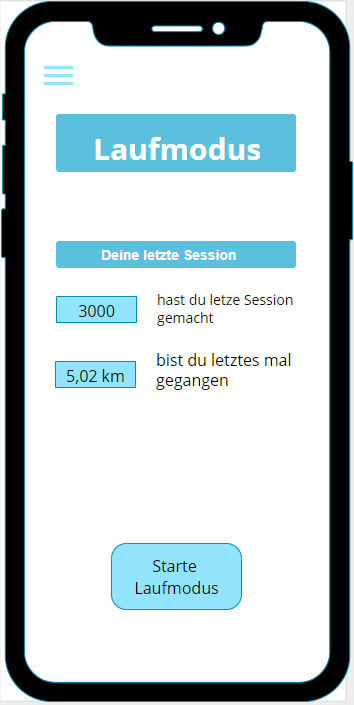
\includegraphics[width=4cm,height=9cm]{./Benutzeroberflaeche/Laufmodus.png}
			\caption{Laufmodus}
			\vspace{30px}
		\end{minipage}
			\hfill
		\begin{minipage}{0.4\textwidth}
			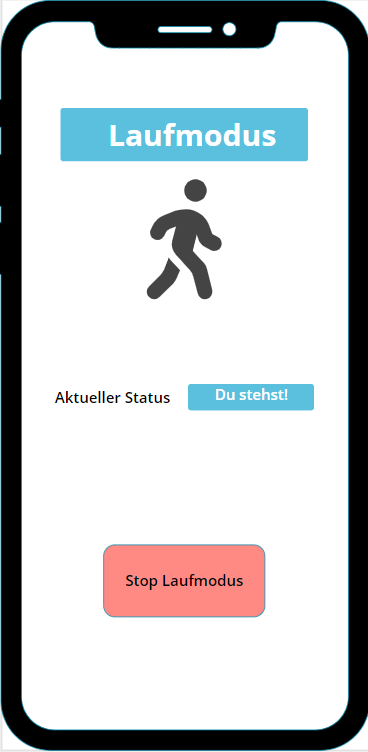
\includegraphics[width=4cm,height=9cm]{./Benutzeroberflaeche/Laufmodus_aktiv.png}
			\caption{aktiver Laufmodus}
			\vspace{30px}
		\end{minipage}
		\begin{minipage}{0.4\textwidth}
			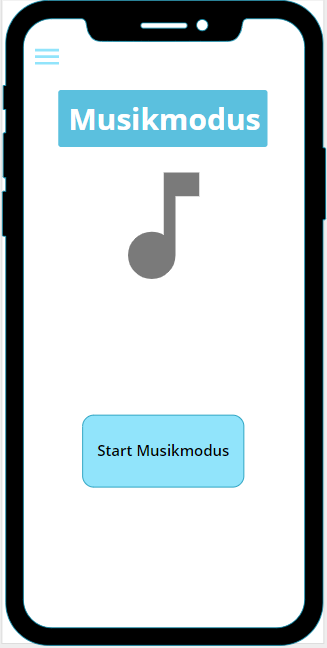
\includegraphics[width=4cm,height=9cm]{./Benutzeroberflaeche/Musikmodus.png}
			\caption{Musikmodus}
		\end{minipage}
		\hfill
		\begin{minipage}{0.4\textwidth}
			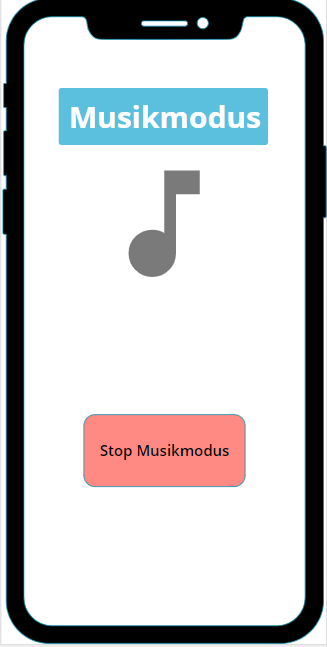
\includegraphics[width=4cm,height=9cm]{./Benutzeroberflaeche/Musikmodus_aktiv.png}
			\caption{aktiver Musikmodus}
			
		\end{minipage}
\end{figure}

\begin{figure}[ht!]
	
	\centering
	\begin{minipage}{0.4\textwidth}
		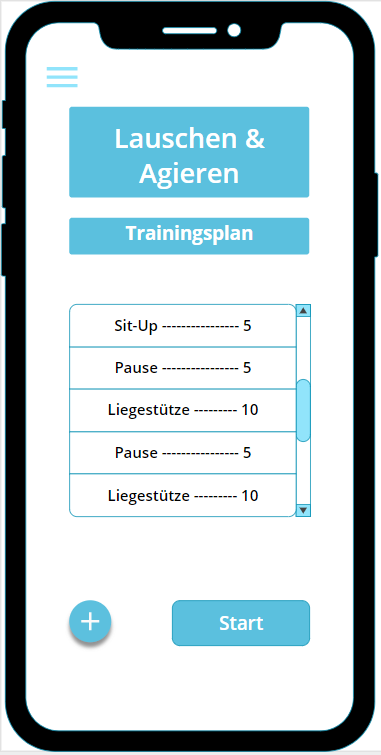
\includegraphics[width=4cm,height=9cm]{./Benutzeroberflaeche/Lauschen_und_Agieren.png}
		\caption{Lauschen und Agieren}
		\vspace{30px}
	\end{minipage}
	\hfill
	\begin{minipage}{0.4\textwidth}
		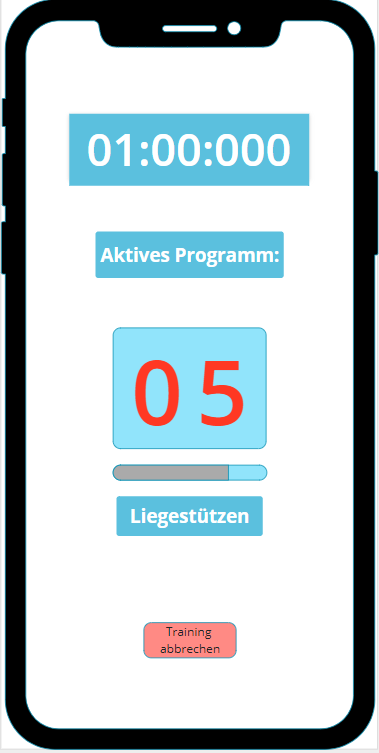
\includegraphics[width=4cm,height=9cm]{./Benutzeroberflaeche/Lauschen_und_Agieren_aktiv.png}
		\caption{Lauschen und Agieren aktiv}
		\vspace{30px}
	\end{minipage}
	\begin{minipage}{0.4\textwidth}
		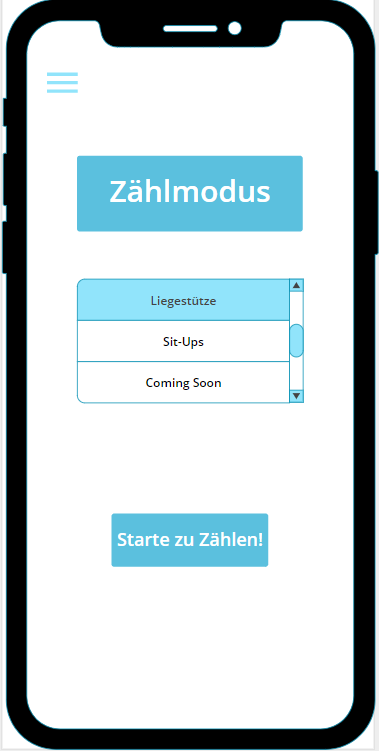
\includegraphics[width=4cm,height=9cm]{./Benutzeroberflaeche/Zaehlmodus.png}
		\caption{Zählmodus}		
	\end{minipage}
	\hfill
	\begin{minipage}{0.4\textwidth}	
		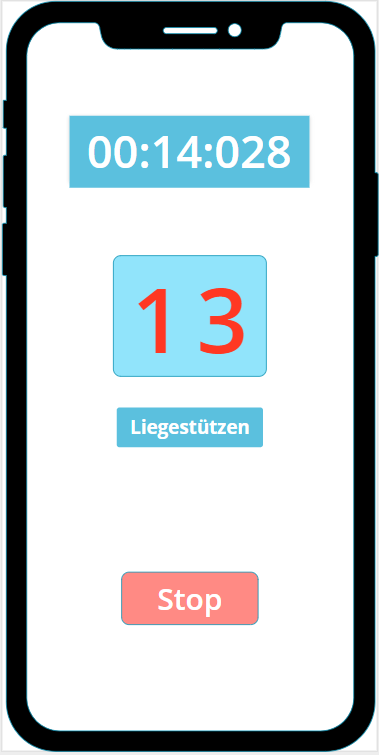
\includegraphics[width=4cm,height=9cm]{./Benutzeroberflaeche/Zaehlmodus_aktiv.png}
		\caption{Zählmodus aktiv}
		
	\end{minipage}
\end{figure}
\begin{figure}[ht!]
	\centering
	\begin{minipage}{0.4\textwidth}
		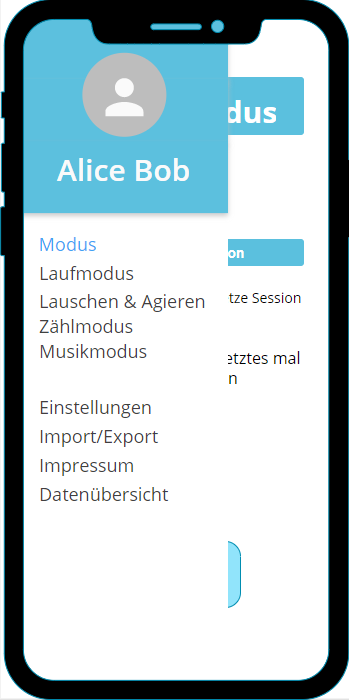
\includegraphics[width=4cm,height=9cm]{./Benutzeroberflaeche/Sidemenu.png}
		\caption{Navigationsmenü}
		\vspace{30px}
	\end{minipage}
	\hfill
	\begin{minipage}{0.4\textwidth}
		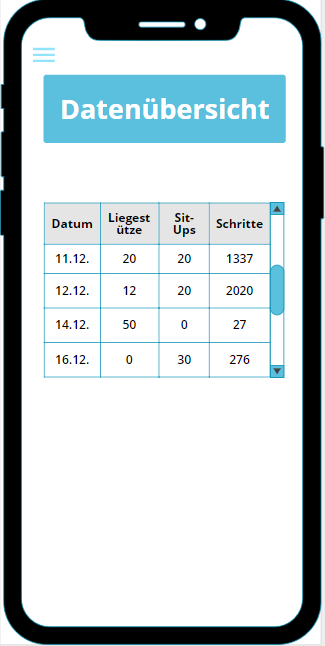
\includegraphics[width=4cm,height=9cm]{./Benutzeroberflaeche/Datenuebersicht.png}
		\caption{Datenübersicht}
		\vspace{30px}
	\end{minipage}
	\begin{minipage}{0.4\textwidth}
		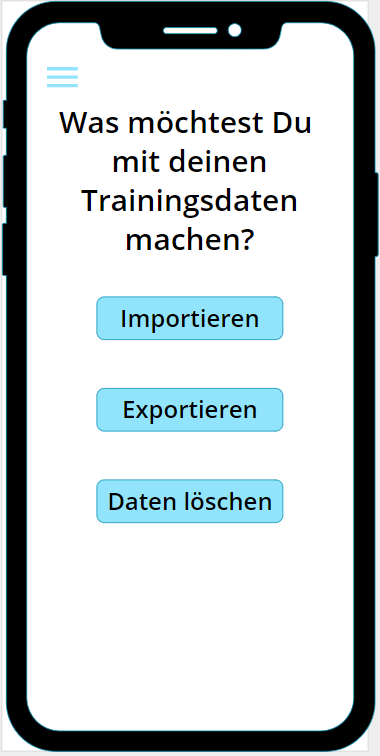
\includegraphics[width=4cm,height=9cm]{./Benutzeroberflaeche/Import_Export.png}
		\caption{Import und Export}
	\end{minipage}
	\hfill
	\begin{minipage}{0.4\textwidth}
		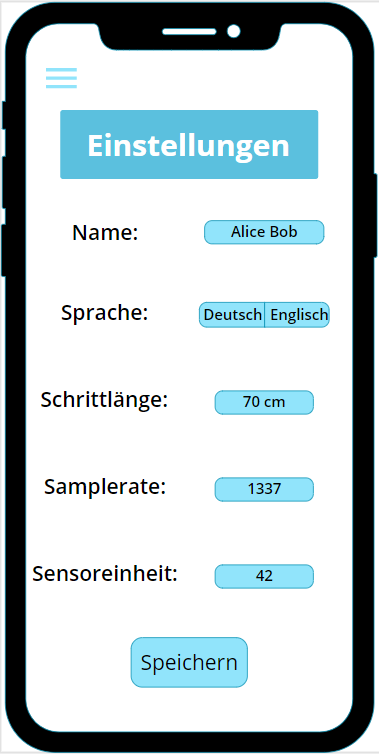
\includegraphics[width=4cm,height=9cm]{./Benutzeroberflaeche/Settings.png}
		\caption{Einstellungen}
	\end{minipage}
\end{figure}

\clearpage
\begin{figure}[ht!]
	\centering
	\begin{minipage}{0.4\textwidth}
		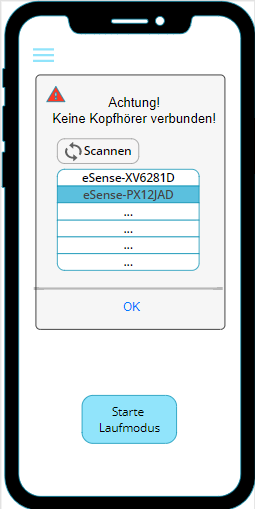
\includegraphics[width=4cm,height=9cm]{./Benutzeroberflaeche/VerbindungsPopUp.png}
		\caption{VerbindungsPop-up}
		\vspace{30px}
	\end{minipage}
\end{figure}
\subsection{Erläuterungen zur Benutzeroberfläche}
\begin{itemize}
  \item Das Auswahlmenü der Modi wird über ein Hamburgermenü realisiert (Button links oben, der ein Menü auf der linken Seite öffnet)
  \item Jeder Modus verfügt über einen einheitlichen Button, der unten mittig liegt und für das Starten und Stoppen eines Vorgangs zuständig ist.
  \item {Das VerbindungsPop-Up (Abb. 13) erscheint, wenn 
  \begin{itemize}
    \item die App gestartet wird,
    \item die BLE-Verbindung unterbrochen wurde,
    \item wenn ein Vorgang gestartet werden soll oder andere Aktivitäten erfolgen (z.b. \Gls{Steuerungsparameter} anpassen), aber gerade keine BLE-Verbindung existiert.
  \end{itemize}
  Die Pop-Up Meldung kann über einen Button jederzeit ausgeblendet werden. 
  Wird eine BLE-Verbindung erfolgreich hergestellt, verschwindet das Pop-Up.
  }
  \item Im Modus Lauschen und Agieren (Abb. 5) wird der Trainingsablaufplan als Liste angezeigt. Die einzelnen Elemente sind in dieser Ansicht manipulierbar, d.h. der Nutzer kann die Reihenfolge der Elemente tauschen und die einzelnen Elemente löschen. Diese Funktionen können z.B. durch gedrückt halten der Elemente oder durch Buttons realisiert werden.
\end{itemize}
Die genannten Punkte erhöhen die Nutzerfreundlichkeit, da die verschiedenen Modi so ähnlich zu bedienen sind und der den Nutzern hoffentlich bekannte Navigationsweg über das Menü intuitiv erscheint.
\section{Qualitätszielbestimmungen}
Der erste Bestandteil des Projekts ist die Bibliothek mit dem Erweiterungsmodul. Diese sollen als Open Source Projekt einer breiteren Entwicklergemeinschaft zur Verfügung gestellt werden, daher legen wir besonderen Wert auf die Korrektheit und Zuverlässigkeit.\\
Dagegen ist bei der App hauptsächlich die Benutzerfreundlichkeit wichtig, während die Robustheit und Zuverlässigkeit der App keine so große Rolle spielen. Generell ergeben sich insgesamt folgende Prioritäten:\\
\begin{tabular}[t]{|c|c|c|c|c|c|}
  \hline
  \textbf{Kriterium} & \textbf{Sehr Wichtig} & \textbf{Wichtig} & \textbf{Weniger Wichtig} & \textbf{Unwichtig}\\
  \hline
  \hline
  Korrektheit & x & & &\\ %%sehr
  \hline
  Zuverlässigkeit & & x & &\\ %%wichtig
  \hline
  Robustheit & & & x &\\  %%weniger
  \hline
  Effizienz & & x & &\\ %%wichtig
  \hline
  Benutzerfreundlichkeit & x & & &\\ %%sehr
  \hline
  Vertrauenswürdigkeit & & & x &\\ %%un
  \hline

\end{tabular}
\vspace{1cm}
\section{Globale Testfälle und Szenarien}
Die Testfälle sollen sicherstellen, dass alle funktionalen Anforderungen korrekt implementiert und umgesetzt wurden.
Die Nummerierung der globalen Testfälle richtet sich nach der Nummerierung der funktionalen Anforderungen.\\
Die Szenarien werden verwendet, um alle geforderten und optionalen Funktionen im Kontext einer Nutzerinteraktion zu testen.\\
Erst nach dem Bestehen aller hier aufgeführten Tests und Szenarien ist das Produkt bereit für die Abnahme.
%%TODO David
  \subsection{Globale Testfälle}
  \subsubsection{Mussanforderungen}
  \paragraph{Bibliothek}
  \begin{itemize}
    \item[/T010/] Bei Aufruf der entsprechenden Schnittstelle der Bibliothek werden plausible Rohdaten in \Gls{Echtzeit} zurückgegeben.
    \item[/T030/] Steuerungsparameter werden geändert. 
    \item[/T040/] Die Datenaufnahme des \Gls{IMU} wird gestartet.
    \item[/T050/] Die Datenaufnahme des \Gls{IMU} wird gestoppt.
  \end{itemize}
  \paragraph{Erweiterungsmodul}
  \begin{itemize}
    \item[/T060/] Der Nutzer tätigt einen Schritt.
    \item[/T061/] Der Nutzer läuft mit einem Schritt pro Sekunde.
    \item[/T062/] Der Nutzer tätigt drei Schritte.
    \item[/T063/] Der Nutzer läuft einen Meter.
  \end{itemize}
  \paragraph{App}
    \begin{itemize}
    \item[/T070/] Der Nutzer startet die App über sein Smartphone und landet im Laufmodus.
    \item[/T075/] Der Nutzer startet den modusspezifischen \Gls{Vorgang}.
    \item[/T080/] Der Nutzer stoppt den modusspezifischen \Gls{Vorgang}. Ihm wird das Vorgangsresultat angezeigt.
    \item[/T090/] Der Nutzer wechselt über ein einblendbares Menü den Modus.
    \item[/T100/] Der Nutzer sieht, ob er gerade \glqq läuft\grqq{} oder \glqq steht\grqq{}.
    \item[/T101/] Die App zeigt die \gls{Schrittfrequenz} im Modus \glqq{}Laufmodus\grqq{} an, sobald der Laufmodus gestartet wird.
    \item[/T102/] Die App zeigt die Schrittanzahl im Modus \glqq{}Laufmodus\grqq{} an, sobald der Laufmodus gestartet wird.
    \item[/T104/] Die App befindet sich im Laufmodus und der Laufmodus ist noch nicht gestartet. Es wird angezeigt, wie viele Schritte der Nutzer beim letzten Vorgang gemacht hat und welche Strecke er dabei zurückgelegt hat.   
    \item[/T140/] Der Nutzer startet die App und verbindet sich mit Hilfe des Pop-ups mit den \gls{Earables}.
    \item[/T150/] Das Smartphone verliert seine Verbindung zu den \gls{Earables} und das Pop Up erscheint.
    \item[/T160/] Der Nutzer klickt das Pop Up weg.
    \item[/T165/] Das Smartphone besitzt keine Verbindung zu den \gls{Earables} und der Nutzer startet einen Vorgang. Das Pop-Up erscheint und der Vorgang wird nicht gestartet.
  \end{itemize}

\subsubsection{Wunschanforderungen}
  \paragraph{Erweiterungsmodul}
    \begin{itemize}
    \item[/T170/] Der Nutzer macht einen Sit-up. 
    \item[/T180/] Der Nutzer macht eine Liegestütze.
  \end{itemize}
  \paragraph{App}
  \begin{itemize}
    \item[/T200/] Die Liegestützen oder Sit-ups werden von der App gezählt und im Modus \glqq{}Zählmodus \grqq{} angezeigt.
    \item[/T210/] Der Nutzer bleibt stehe, die Musik stoppt. Der Nutzer läuft weiter, die Musik läuft weiter.
    \item[/T221/] Der Nutzer stellt einen Trainingsablaufplan zusammen.
    \item[/T222/] Die App gibt dem Nutzer über Sprachanweisung aus was die nächste Übung ist.
    \item[/T223/] Nach Vorgangsende wird die benötigte Zeit angezeigt.
    \item[/T250/] Der Nutzer ändert seinen Namen.
    \item[/T260/] Der Nutzer ändert die Sprache auf Englisch.
    \item[/T265/] Der Nutzer ruft erstmals die App auf, diese passt sich seiner Systemsprache an.
    \item[/T270/] Der Nutzer löscht Vorgangsdaten.
    \item[/T280/] Der Nutzer verändert die Samplingrate.
    \item[/T285/] Der Nutzer ändert die Schrittlänge.
    \item[/T290/] Der Nutzer ruft erstmals die App auf, er wird aufgefordert seinen Namen und seine Schrittlänge zu setzen.
    \item[/T300/] Der Nutzer importiert seine Vorgangsdaten aus einer CSV-Datei.
    \item[/T320/] Der Nutzer sieht sich die gespeicherten Trainingsdaten an.
   \end{itemize}
   
  \subsection{Szenarien}
	Vor jedem Szenario wird davon ausgegangen, dass das Smartphone angeschaltet ist und die App noch nicht gestartet wurde. Des weiteren wird angenommen, dass die App nicht zum ersten mal gestartet wird, außer bei dem Szenario \glqq{}Erstnutzung\grqq{}.
    \subsubsection{Mussanforderungen}
      \paragraph{Laufmodus}
      \begin{enumerate}
        \item Der Nutzer startet die App. (/T070/)
        \item Der Nutzer verbindet in der App die \gls{Earables}, über \gls{BLE} mit seinem Smartphone.
        \item Nach dem Startvorgang der App wird in den Modus \glqq Laufmodus\grqq{} gewechselt.
        \item Falls es schon einen Laufvorgang zuvor gab, werden nun die Anzahl der zurückgelegten Schritte und die zurückgelegte Distanz angezeigt. (/T104/)
        \item Die \Gls{Earables} werden korrekt am Ohr des Nutzers angebracht.
        \item Der Nutzer startet den Laufmodus.
        \item Die App zeigt dem Nutzer den Status \glqq stehend\grqq{} an.
        \item Die App zeigt dem Nutzer die aktuelle \gls{Schrittfrequenz} und die Anzahl der bisher zurückgelegten Schritte an. (/T101/, /T102/)
        \item Sobald der Nutzer anfängt zu gehen zeigt die App \glqq gehend\grqq{} an.
        \item Sobald der Nutzer wieder still steht ändert sich der Zustand wieder zurück zu \glqq stehend\grqq. 
      \end{enumerate}

    \subsubsection{Wunschanforderungen}

    
    \paragraph{Zählmodus}
      \begin{enumerate}
        \item Der Nutzer startet die App. (/T070/)
        \item Der Nutzer verbindet in der App die \gls{Earables}, über \gls{BLE} mit seinem Smartphone..
        \item Nach dem Startvorgang der App wechselt der Nutzer in den Modus \glqq Zählmodus\grqq . (/T090/)
        \item Die \Gls{Earables} werden korrekt am Ohr des Nutzers angebracht.
        \item Der Nutzer wählt eine verfügbare Übung aus. 
        \item Der Nutzer startet den gewählten \Gls{Vorgang}.
        \item Der Nutzer führt die Übung 15 (natürliche Zahl) mal aus.
        \item Der Nutzer stoppt den laufenden \Gls{Vorgang}.
        \item Die App zeigt 15 an. (/T200/)
      \end{enumerate}

    
    \paragraph{Start/Stop Musikmodus}
      \begin{enumerate}
        \item Der Nutzer startet die App. (/T070/)
        \item Der Nutzer verbindet in der App die \gls{Earables}, über \gls{BLE} mit seinem Smartphone.
        \item Der Nutzer spielt Musik mit der vorinstallierten Musik-App ab.
        \item Nach dem Startvorgang der App wechselt der Nutzer in den Modus \glqq Laufmodus\grqq . (/T090/)
        \item Die \Gls{Earables} werden korrekt am Ohr des Nutzers angebracht.
        \item Der Nutzer beginnt zu gehen.
        \item Der Nutzer startet den gewählten \Gls{Vorgang}.
        \item Der Nutzer hört auf zu gehen.
        \item Die Musik wird pausiert. (/T210/)
        \item Der Nutzer geht weiter.
        \item Die Musik startet automatisch wieder. (/T210/)
      \end{enumerate}
  
      \paragraph{Lauschen\&Agieren}
      \begin{enumerate}
        \item Der Nutzer startet die App. (/T070/)
        \item Der Nutzer verbindet in der App die \gls{Earables}, über \gls{BLE} mit seinem Smartphone.
        \item Nach dem Startvorgang der App wechselt der Nutzer in den Modus \glqq Lauschen\&Agieren\grqq . (/F090/)
        \item Die \Gls{Earables} werden korrekt am Ohr des Nutzers angebracht.
        \item Der Nutzer stellt sich ein Training aus den verfügbaren Übungen zusammen (/T221/).
        \item Der Nutzer startet den gewählten \Gls{Vorgang}.
        \item Dem Nutzer wird per \Gls{TTS} die aktuelle Übung angesagt (/T222/).
        \item Der Nutzer führt die Übung aus.
        \item Die letzten beiden Schritte werden so lange wiederholt, bis alle ausgewählten Übungen erledigt sind.
        \item Der \Gls{Vorgang} wird automatisch beendet.
        \item Die App zeigt die benötigte Zeit für den Vorgang an (/T223/).
      \end{enumerate}

      \paragraph{Einstellungen}
      \begin{enumerate}
        \item Der Nutzer startet die App. (/T070/)
        \item Der Nutzer verbindet in der App die \gls{Earables}, über \gls{BLE} mit seinem Smartphone.
        \item Nach dem Startvorgang der App wechselt der Nutzer in die Ansicht \glqq Einstellungen\grqq .
        \item Der Nutzer ändert seinen Namen (/T250/).
        \item Der Nutzer ändert die Sprache auf Englisch (/T260/).
        \item Dem Nutzer löscht die gespeicherten \Gls{Vorgangsdaten} (/T270/).
        \item Dem Nutzer ändert die Samplingrate (/T280/).
        \item Der Nutzer ändert seine Schrittlänge (/T285/).
        \item Der Nutzer beendet die App.
        \item Der Nutzer startet die App. (/T070/)
        \item Der Nutzer wechselt in die Ansicht \glqq Einstellungen\grqq .
        \item Die Einstellungen sind exakt so, wie sie vorher eingestellt wurden.
      \end{enumerate}

      \paragraph{Erstnutzung}
      \begin{enumerate}
        \item Der Nutzer startet die App zum ersten Mal. 
        \item Der Nutzer wird aufgefordert seinen Namen und seine Schrittlänge zu setzen. (/T290/)
        \item Der Nutzer wählt im Hamburgermenü den Reiter Einstellungen aus.
        \item Der Nutzer ändert die Sprache auf Englisch.(/T260/)
        \item Danach wechselt der Nutzer in den \glqq Laufmodus\grqq.
        \item Der Nutzer schließt die App.
        \item Der Nutzer startet die App erneut und befindet sich nun im \glqq Laufmodus\grqq. (/T070/)
        \item Sein Name, seine Schrittlänge und die in-App Sprache wurden gespeichert.
      \end{enumerate}

      \paragraph{Vorgangsdaten importieren/exportieren}
      \begin{enumerate}
        \item Der Nutzer startet die App. (/T070/)
        \item Der Nutzer wählt über das Hamburgermenü den Reiter \glqq{}Import/Export \grqq{}.
        \item Der Nutzer exportiert seine Daten. 
        \item Der Nutzer löscht seine Daten. (/T270/)
        \item Der Nutzer importiert seine Daten aus einer CSV-Datei. (/T300/)
        \item Die Daten sind alle wieder vorhanden so als ob der Nutzer sie nie gelöscht hätte.
      \end{enumerate}

    \paragraph{Trainingsdaten anschauen}
    \begin{enumerate}
	\item Der Nutzer startet die App. (/T070/)
 	\item Der Nutzer wechselt über das Hamburgermenü in die Datenübersicht.
	\item Dem Nutzer werden die letzten Trainingsdaten der letzten 30 Vorgangstage angezeigt. (/T320/)
    \end{enumerate}

    \paragraph{Pop-up}
    \begin{enumerate}
	\item Der Nutzer startet die App. (/T070/)
 	\item Das Pop-up Fenster erscheint.
 	\item Der Nutzer klickt das Pop-up weg. (/T160/)
 	\item Der Nutzer versucht einen Laufvorgang zu starten.
 	\item Das Pop-up erscheint. 
 	\item Der Nutzer stellt eine Verbindung zu den \gls{Earables} her.
 	\item Der Nutzer entfernt sich mit seinem Smartphone von de \gls{Earables}.
 	\item Das Smartphone verliert die Bluetooth Verbindung zu den \gls{Earables} und das Pop-up erscheint. (/T150/)
    \end{enumerate}

\section{Entwicklungsumgebung}
Wir arbeiten an dem Projekt mit Visual Studio 2017 oder neuer, sodass alle eine einheitliche Entwicklungsumgebung verwenden.\\
Dabei kommt der .NET Standard 2.0 zum Einsatz, der C\# 7.2 verwendet. Wir arbeiten außerdem mit Xamarin Forms.\\
Zur Versionskontrolle und zur Projektübersicht wird Git verwendet, das Repository liegt öffentlich auf Github\footnote{\url{https://github.com/vlle1/earablesKIT}}.
\clearpage
\printglossaries
\stepcounter{section}
\end{document}
